%
% ritzAufProblem.tex 
%
% 
%
% !TEX root = ../../buch.tex
% !TEX encoding = UTF-8
%



\section{Ritz Verfahren angewandt\label{antennen:ritzAnw}}


Wie in REF erwähnt konnten wir dank der Symmetrie das Problem nur auf eine Ecke abbilden. Diese Ecke setze man nun geschickt wie in der Abbildung \ref{antennen:koordSysBsp} zu sehen in ein Koordinatensystem.

%TODO bild ist weit weg [htbp] ILLEGAL
\begin{figure}[htbp]
	\centering
	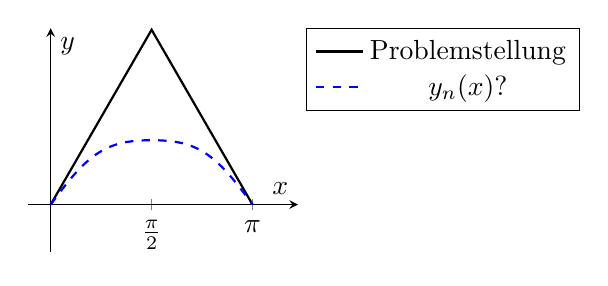
\begin{tikzpicture}
		\begin{axis}[
			scale=0.5,
			axis lines=middle,
			xlabel={$x$},
			ylabel={$y$},
			xtick={0, 1.5708, 3.14159},
			xticklabels={0, $\frac{\pi}{2}$, $\pi$},
			ytick=\empty,
			enlargelimits,
			clip=false,
			xmin=0, xmax=3.5,
			ymin=0, ymax=2,
			domain=0:pi, 
			samples=100,
			legend pos=outer north east,
			axis equal
			]
			% 3eck spitze
			\addplot[thick] coordinates {(0,0) (1.5708, pi*1.732/2) (3.14159, 0)};
			\addlegendentry{Problemstellung}
			
			\addplot[thick, blue, dashed, domain=0:3.14159, samples=100] {1.0882345*sin(deg(x))+0.0866761*sin(3*deg(x))};
			\addlegendentry{$y_n(x)?$}
		\end{axis}
	\end{tikzpicture}
	\caption{Problemstellung im Koordinatensystem}
	\label{antennen:koordSysBsp}
\end{figure}
Um die Effizienz $\eta$ zu optimieren, müssen wir mit der Approximationsfunktion
$y_n(x)$, wie in REF %~\ref{an} 
erwähnt, die quadrierte Fläche $A$ maximieren und die Länge $l$ minimieren.


\subsection{Nebenbedingungen von $y_n(x)$\label{antenennen:nebenbedRitz}}

Eine Nebenbedingung ist es, dass bei $y_n(0)$ und $y_n(\pi)$ die Funktion null sein muss.
Diese Nebenbedingung ist sehr wichtig für die Stetigkeit der finalen Form die wir optimieren.

Die Sinus-Fourier Reihe \eqref{antennen:unserRitz} hat eine weitere gute Eigenschaft, 
welche klar wird, wenn man in das gleiche Koordinatensystem wie bei der Abbildung \ref{antennen:koordSysBsp}
benützt und $y_n(x)$ mit beispielsweise den Koeffizienten $a_1=a_2=1$ plottet.

%TODO bild ist weit weg [htbp] ILLEGAL
\begin{figure}[htbp]
	\centering
	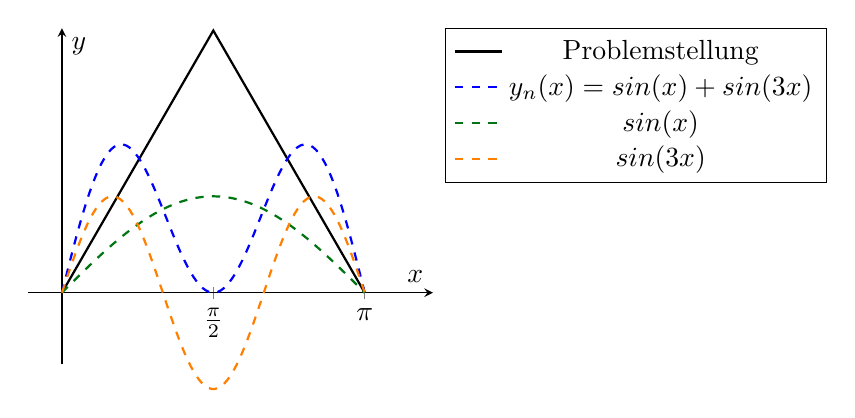
\begin{tikzpicture}
		\definecolor{clr1}{RGB}{0, 117, 18}
		\begin{axis}[
			scale=0.75,
			axis lines=middle,
			xlabel={$x$},
			ylabel={$y$},
			xtick={0, 1.5708, 3.14159},
			xticklabels={0, $\frac{\pi}{2}$, $\pi$},
			ytick=\empty,
			enlargelimits,
			clip=false,
			xmin=0, xmax=3.5,
			ymin=0, ymax=2,
			domain=0:pi, 
			samples=100,
			legend pos=outer north east,
			axis equal
			]
			% 3eck spitze
			\addplot[thick] coordinates {(0,0) (1.5708, pi*1.732/2) (3.14159, 0)};
			\addlegendentry{Problemstellung}
			
			\addplot[thick, blue, dashed, domain=0:3.14159, samples=100] {sin(deg(x))+sin(3*deg(x))};
			\addlegendentry{$y_n(x) = sin(x)+sin(3x)$}
			
			\addplot[thick, clr1, dashed, domain=0:3.14159, samples=100] {sin(deg(x))};
			\addlegendentry{$sin(x)$}
			
			\addplot[thick, orange, dashed, domain=0:3.14159, samples=100] {sin(3*deg(x))};
			\addlegendentry{$sin(3x)$}
		\end{axis}
	\end{tikzpicture}
	\caption{Nebenbedingungen im Koordinatensystem}
	\label{antennen:nebenbedGrafik}
\end{figure}

In der Abbildung \ref{antennen:nebenbedGrafik} ist zu sehen, dass dank der Punktsymmetrie 
der ungeraden Sinus-Funktionen, die Nebenbedingungen
\begin{equation}
	\begin{aligned}
		y_n(0)
		&=
		0
		\\
		y_n(\pi)
		&=
		0
	\end{aligned}
\label{antennen:nebenbed3eck}
\end{equation}
\em immer \em als \em erfüllt \em zu betrachten sind. Im weiteren Verlaufen werden diese 
Nebenbedingungen somit nicht mehr beachtet.

\subsection{Die Lagrangefunktion \label{antennen:lagrangeFunktionen}}

%Die beste Fläche ist auch gerade die beste Fläche im quadrat \qed

Abstrahieren wir das Problem nun ein bisschen. Anstelle der Fläche $A$, reden wir nun von 
der Funktion $f$ und Länge $l$ wird zur Nebenbedingung $n$. 

An dieser Stelle sind unsere Koeffizienten $a_k$ konkret zu bestimmen. 
Somit sind die neu erwähnten Funktionen 

\begin{equation}
\begin{aligned}
	A
	\rightarrow
	f(a_1,\ldots,a_k)
	\rightarrow
	f(a_1,a_2)
	&=
	\int\limits_{0}^{\pi} y_n(x,a_1,a_2)\, dx
	\\
	l
	\rightarrow
	n(a_1,\ldots,a_k)
	\rightarrow
	n(a_1,a_2)
	&=
	\int\limits_{0}^{\pi} \sqrt{\frac{d}{d x} y_n\left(x, a_1, a_2\right)+1}\, dx
\end{aligned}
\label{antennen:lagrangeNamen}
\end{equation}


auch in deren Abhängigkeit bei \eqref{antennen:lagrangeNamen} zu sehen. 

Die Fläche unter der Kurve ergibt sich aus dem Integral der Funktion, 
während die Länge, also der obere Rand der Funktion, durch die in Kapitel REF  %\ref{label} 
erläuterte Formel berechnet wird. 

Die Nebenbedingung $n$ setzen wir nun gleich einer Konstanten Länge $\ell$
\begin{equation}
n(a_1, a_2)
=
\ell
\label{antennen:constNebenbed}
\end{equation}

und wie jede gute Nebenbedingung setzen wir diese noch gleich null

\begin{equation}
\begin{aligned}
	n(a_1, a_2) - \ell
	&=
	0
	\\
	n(a_1, a_2, \ell)
	&=
	0
\label{antennen:fertigeNebenbed}
\end{aligned}
\end{equation}

Nun kann man die Lagrangefunktion
\begin{equation}
L(x,a_1,a_2,\lambda)
= 
f(a_1,a_2)+\lambda \: n(a_1,a_2, \ell)
\end{equation}

definieren. Dazu wird die Funktion $f$ mit der Lagrange-Nebenbedingung $\lambda \: n$ addiert. 
Mehr zu der Lagrangefunktion findet man unter dem Kapitel REF %\ref{label}

\subsection{Lagrange Gleichungssystem\label{antennen:lagrangeGLsys}}

Nun möchte man die Lagrangefunktion $L$ ableiten und 0 setzen. Nur heisst das in
diesem Kontext

% TODO GLsys bisschen spacen
\begin{equation}
	\nabla L = \vec{0} 
	\left\{ 
	\begin{aligned}
		\frac{\partial L}{\partial a_1} = 0 \\
		\frac{\partial L}{\partial a_2} = 0 \\
		\frac{\partial L}{\partial \lambda} = 0
	\end{aligned}
	\right.
	\label{antennen:lagrangeGrad}
\end{equation}

den Gradienten berechnen und dem Nullvektor gleichsetzen. Dabei entsteht hier ein 
$n+1$ dimensionales Gleichungssystem \eqref{antennen:lagrangeGrad}

An dieser Stelle soll es einem bewusst werden, was dieses Kapitel von anderen 
unterscheidet. Dank dem Verfahren nach Ritz konnten wir ein unendlich dimensionales
Problem, in ein endlich dimensionales verwandeln. 
Konkret heisst es, dass wir keine Differentialgleichung lösen müssen, sondern, 
das Gleichungssystem, welches wir bei \eqref{antennen:lagrangeGrad} erhalten haben.

Somit sieht das Gleichungssystem \eqref{antennen:lagrangeGrad}

\begin{equation}
	\begin{aligned}
		\int_0^\pi \sin (x) dx
		&=
		-\lambda \int_0^\pi \frac{\left(a_1 \cos (x)+3 a_2 \cos (3 x)\right) 
			\cos (x)}{\sqrt{\left(a_1 \cos (x)+3 a_2 \cos (3 x)\right)^2+1}} \, dx \\
		\int_0^\pi \sin (3 x) dx
		&=
		-\lambda \int_0^\pi \frac{3\left(a_1 \cos (x)+3 a_2 \cos (3 x)\right) 
			\cos (3 x)}{\sqrt{\left(a_1 \cos (x)+3 a_2 \cos (3 x)\right)^2+1}} \, dx \\
		\ell
		&=
		\int_0^\pi \sqrt{\left(a_1 \cos (x)+3 a_2 \cos (3 x)\right)^2+1} \, dx
	\end{aligned}
\label{antennen:lagrangeGradKonkret}
\end{equation}

in diesem Fall mit 2 Koeffizienten konkret so \eqref{antennen:lagrangeGradKonkret} aus.

\subsection{Das Gleichungssystem Lösen\label{antennen:glSysSolve}}

Ein gutes Verfahren, was sich hierbei anbieten wäre das Gradienten-abstiegs/anstiegs-Verfahren. 











